\section{One-bit Digital Comparator}
\subsection{Introduction}%Purpose, brief intro, Contribution
    \subsubsection{Background}
    The one-bit comparator can perform a logic comparison to judge the magnitude of 
    two single-bit inputs. 
    It outputs three different states to show the result 
    which indicates greater, smaller, and equal.
    \subsubsection{Purpose}
    In this experiment, we aimed to design a circuit that is able to compare two one-bit inputs and give three different states of output, which shows the numerical relationship between two inputs.
    \subsubsection{Design and Key-results}
    \subsubsection{Contribution}

\subsection{Materials and Methods}%Show FPGA solution
    \subsubsection{Structure Block Diagram}
    \begin{figure}[h]
        \centering
        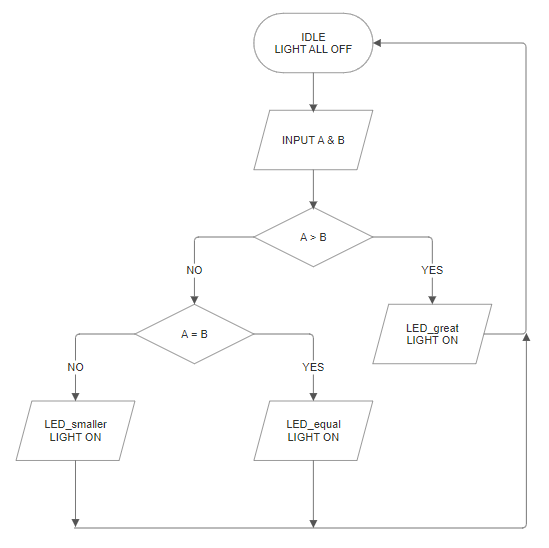
\includegraphics[width=0.8\linewidth]{Structure_Block_Diagram/onebitcomparator_BlockStructureDiagram.png}
        \label{obc_SBD}
    \end{figure}
    \FloatBarrier
    \subsubsection{Truth Table}
    \begin{table}[h]
    \centering
        \begin{tabular}{|l|l|l|l|l|}
        \hline
        A & B & LED\_greater & LED\_equal & LED\_smaller \\ \hline
        0 & 0 & 0            & 1          & 0            \\ \hline
        0 & 1 & 0            & 0          & 1            \\ \hline
        1 & 0 & 1            & 0          & 0            \\ \hline
        1 & 1 & 0            & 1          & 0            \\ \hline
        \end{tabular}
    \end{table}
    \FloatBarrier
    \subsubsection{Signal Waveforms}
    \begin{figure}[h]
        \centering
        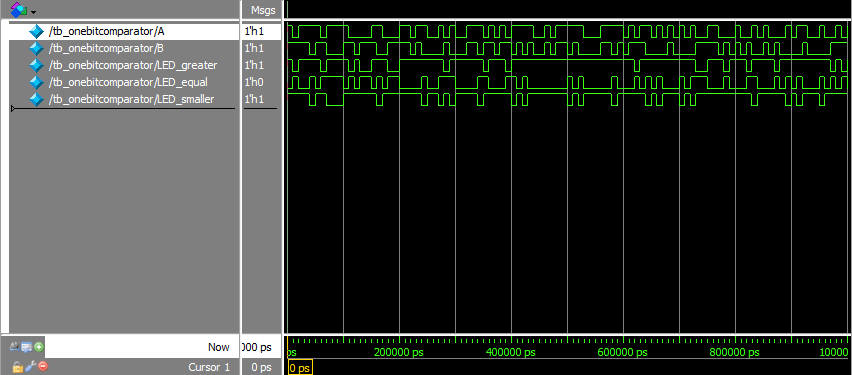
\includegraphics[width=0.8\linewidth]{Testbench_Waveform/tb_onebitcomparator_waveform.png}
        \label{tb_obc}
    \end{figure}
    \FloatBarrier
    \subsubsection{Resources in Board}

\subsection{Results}%Show simulation and corresponding test results
    \subsubsection{Testbench}
    In this experiment, the testbench was built to accept two one-bit inputs. The testing inputs were randomly generated, and the outputs were presented by waveform. The expected outputs are shown below:
    \begin{enumerate}
        \item Input A
    \end{enumerate}
\subsection{Discussions and Conclusion}
    \subsubsection{Discussions}%This is an optional bonus part, it is not essential.
    During this experiment, we encountered a problem of differences in the 
    recognition of signal inputs. When the button is pressed, 
    we expect it is inputting signal 1 into the system. 
    However, instead of entering signal 1, the chip recognizes the button 
    pressing behaviour as sending signal 0. Eventually, the misinterpretation 
    resulted in the opposite output. 
    To fix this output error, we decided to reverse the logic judgment 
    that was used to compare the input signals. 
    Now, when the chip accepts the input A<B, which we originally predicted 
    as A>B, it correctly produces the expected outcome of A>B. 
    %Found this problem in the last experiment.

    \subsubsection{Conclusion}
    In this experiment, we met some unexpected errors. Eventually, we overcame them by discussion. We successfully designed a circuit that can compare two single-bit inputs and give a correct magnitude relationship outcome.
\subsection{Appendices} References and Appendices
    \subsubsection{Reference}%This is a list of all the sources cited in the report, formatted according to a specific citation style. You need to use the IEEE reference format (http://journals.ieeeauthorcenter.ieee.org/wpcontent/uploads/sites/7/IEEE_Reference_Guide.pdf).
    \subsubsection{Appendices}%This optional section can include codes, raw data, calculations, additional graphs, and other supplementary material that is relevant but not essential to the main report.